
%(BEGIN_QUESTION)
% Copyright 2006, Tony R. Kuphaldt, released under the Creative Commons Attribution License (v 1.0)
% This means you may do almost anything with this work of mine, so long as you give me proper credit

Suppose an electric oven is equipped with a temperature-sensitive control switch, which is wired to a control relay to send electric power to its heating element:

$$\includegraphics[width=15.5cm]{i01449x01.eps}$$

How would this simple {\it on-off} control system respond to changes in oven temperature, in its effort to maintain temperature at the setpoint?  Be detailed in your explanation of the temperature switch and relay circuit's behavior.  Also sketch a graph of the oven temperature over time:

$$\includegraphics[width=15.5cm]{i01449x02.eps}$$

\underbar{file i01449}
%(END_QUESTION)





%(BEGIN_ANSWER)

A simple {\it on-off} control system will apply full power to the heating element if the temperature is less than the setpoint, and will completely shut off power to the heating element if the temperature is greater than the setpoint.  The result is a temperature graph that oscillates around the setpoint value over time.
 
$$\includegraphics[width=15.5cm]{i01449x03.eps}$$

As you can see, the temperature can never settle at any one temperature, since the control action is all-or-nothing, and changes based on a simple ``greater-than'' or ``less-than'' relationship between the process variable and the setpoint. 

This is an example of a {\it closed-loop} control system.  The control ``loop'' may be represented in the ladder logic schematic by means of causal arrows:

$$\includegraphics[width=15.5cm]{i01449x04.eps}$$


%(END_ANSWER)





%(BEGIN_NOTES)

\vskip 20pt \vbox{\hrule \hbox{\strut \vrule{} {\bf Virtual Troubleshooting} \vrule} \hrule}

This question is a good candidate for a ``Virtual Troubleshooting'' exercise.  Presenting the diagram to students, you first imagine in your own mind a particular fault in the system.  Then, you present one or more symptoms of that fault (something noticeable by an operator or other user of the system).  Students then propose various diagnostic tests to perform on this system to identify the nature and location of the fault, as though they were technicians trying to troubleshoot the problem.  Your job is to tell them what the result(s) would be for each of the proposed diagnostic tests, documenting those results where all the students can see.

During and after the exercise, it is good to ask students follow-up questions such as:

\begin{itemize}
\item{} What does the result of the last diagnostic test tell you about the fault?
\item{} Suppose the results of the last diagnostic test were different.  What then would that result tell you about the fault?
\item{} Is the last diagnostic test the best one we could do?
\item{} What would be the ideal order of tests, to diagnose the problem in as few steps as possible?
\end{itemize}

%INDEX% Control, basics: on/off control
%INDEX% Process: cookie baking oven

%(END_NOTES)


